\section{Конструкторский раздел}
В данном разделе cпроектирована базы данных для проведения футбольных турниров. Была разработана схема базы данных, которая включает в себя таблицы, связи между ними и атрибуты. Каждая таблица в базе данных была описана подробно, описывая ее структуру, включая названия полей и их типы данных. Также были представлены алгоритм расчёта турнирной таблицы и ролевая модель.
\subsection{Проектирование базы данных}
На рисунке \ref{img:db} представлена схема разрабатываемой базы данных.

\begin{figure}
  \centering
  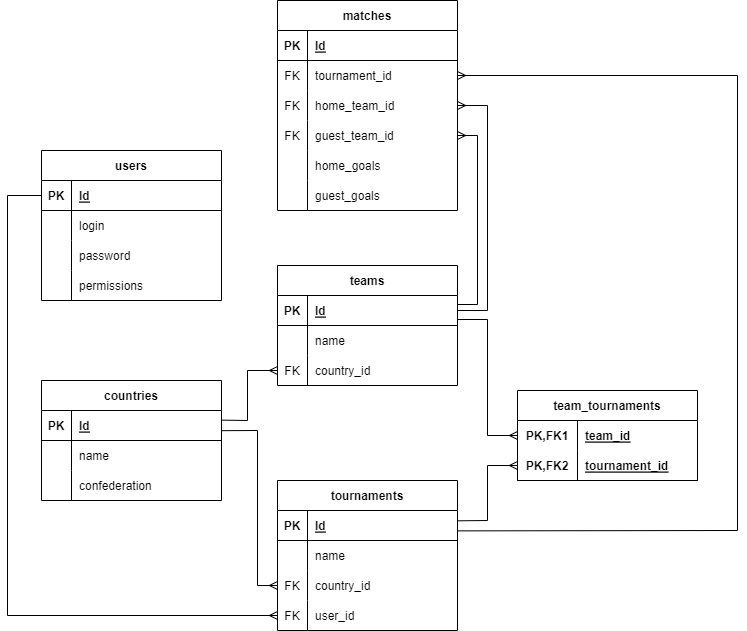
\includegraphics[scale=0.5]{inc/db}
  \caption{Схема разрабатываемой базы данных}
  \label{img:db}
\end{figure}

Таблица users хранит информацию о пользователях и содержит следующие поля:
\begin{itemize}
    \item id --- идентификатор пользователя, первичный ключ; 
    \item login --- логин пользользователя, символьный тип;
    \item password --- hash пароля, символьный тип;
    \item permissions --- права пользователя, символьный тип.
\end{itemize}

Таблица teams хранит информацию о командах и содержит следующие поля:
\begin{itemize}
    \item id --- идентификатор команды, первичный ключ; 
    \item name --- название команды, символьный тип;
    \item country\_id --- идентификатор страны базирования команды, внешний ключ на поле id таблицы countries.
\end{itemize}

Таблица countries хранит информацию о странах и содержит следующие поля:
\begin{itemize}
    \item id --- идентификатор страны, первичный ключ; 
    \item name --- название страны, символьный тип;
    \item confederation --- конфедерация страны, символьный тип.
\end{itemize}

Таблица tournaments хранит информацию о турнирах и содержит следующие поля:
\begin{itemize}
    \item id --- идентификатор турнира, первичный ключ; 
    \item name --- название турнира, символьный тип;
    \item country\_id --- идентификатор страны проведения турнира, внешний ключ на поле id таблицы countries;
    \item user\_id --- идентификатор создателя турнира, внешний ключ на поле id таблицы users.
\end{itemize}

Таблица matches хранит информацию о матчах и содержит следующие поля:
\begin{itemize}
    \item id --- идентификатор матча, первичный ключ; 
    \item tournament\_id --- идентификатор турнира, внешний ключ на поле id таблицы tournaments;
    \item home\_team\_id --- идентификатор домашней команды, внешний ключ на поле id таблицы teams.
    \item guest\_team\_id --- идентификатор гостевой команды, внешний ключ на поле id таблицы teams.
    \item home\_goals --- количество голов домашней команды, целое число;
    \item guest\_goals --- количество голов гостевой команды, целое число.
\end{itemize}
\newpage
Таблица team\_tournaments хранит информацию о связях команда-турнир и содержит следующие поля:
\begin{itemize}
    \item team\_id --- идентификатор команды, внешний ключ на поле id таблицы teams, часть первичного ключа;
    \item tournament\_id --- идентификатор турнира, внешний ключ на поле id таблицы tournament, часть первичного ключа.
\end{itemize}

\subsection{Алгоритм расчёта турнирной таблицы}
При создании базы данных была определена функция get\_table для расчёта турнирной таблицы. Возвращаемая таблица содержит количество матчей, побед, ничьих, поражений, забитых голов, пропущенных голов и очков для каждой команды турнира. Кроме того, таблица сортируется по убыванию по количеству очков. При равенстве очков более высокое место займёт команда с большей разницей голов. В случае равного количества очков и разницы голов выше окажется команда с большим количеством побед.

На рисунке \ref{img:block} представлена схема алгоритма расчёта турнирной таблицы.
\begin{figure}
  \centering
  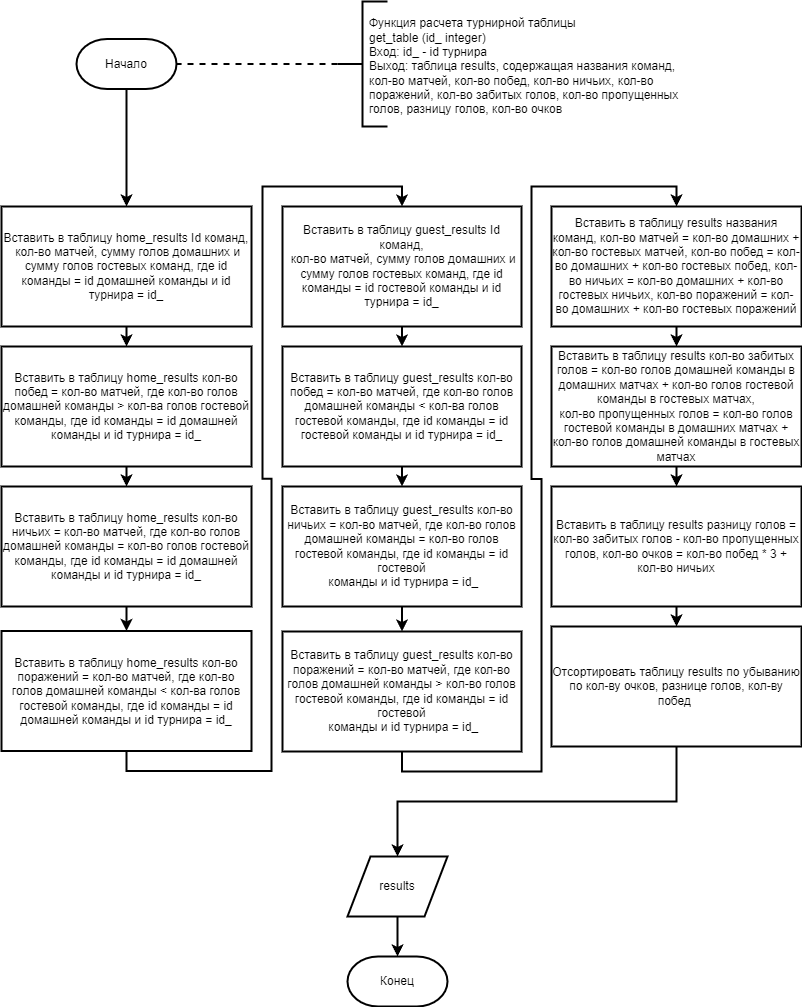
\includegraphics[scale=0.6]{inc/block}
  \caption{Схема алгоритма расчёта турнирной таблицы}
  \label{img:block}
\end{figure}

\subsection{Создание ролевой модели}
Для каждой категории пользователей, описанных ранее, была создана отдельная роль в базе данных.
\begin{enumerate}
    \item Гость имеет права на просмотр всех таблиц. Кроме того, гость имеет права на добавление записей в таблице users для возможности регистрации и авторизации. Другими правами гость не наделён.
    \item Авторизованный пользователь также имеет права на просмотр всех таблиц. У него есть возможность создания команд, турниров и матчей, поэтому авторизованный пользователь наделён правами на добавление записей в таблицы teams, tournaments, team\_tournaments и matches. Кроме того, он может удалять турниры, а также изменять и удалять матчи, поэтому имеет права на удаление записей из таблиц tournaments, matches и team\_tournaments и права на обновление записей в таблице matches.
    \item Администратор имеет права на просмотр, удаление, добавление и обновление записей во всех таблицах.
\end{enumerate}

\subsection*{Вывод}
В данном разделе была спроектирована база данных, в результате чего была приведена схема разрабатываемой базы данных и описаны поля всех таблиц. Также был приведён алгоритм расчёта турнирной таблицы и описаны права доступа для каждой категории пользователей. 

